 \documentclass[book.tex]{subfiles}
\begin{document}
\label{sec:id_software}
Around the same time as the group was rejected by Nintendo, Romero was approached by Scott Miller of Apogee Software. They agreed to make \textit{Commander Keen in Invasion of the Vorticons}, to be published by Apogee Software. The team could not afford to leave their jobs to work on the game full-time, so they continued to work at Softdisk, spending their time on the Gamer's Edge games during the day and on Commander Keen at night and weekends using Softdisk computers.\\

\par
The game was completed in early December 1990 and divided into three episodes: \textit{Marooned on Mars}, \textit{The Earth Explodes}, and \textit{Keen Must Die!}. The game was published as shareware, whereby Marooned on Mars was released for free, and the other two episodes were available for purchase.\\

\par
After the arrival of the first royalty check from Apogee, the team planned to quit Softdisk and start their own company. On February 1, 1991, the team founded \textit{id Software} having four owners: John Carmack, John Romero, Tom Hall and artist Adrian Carmack\footnote{See Masters of Doom, chapter 4}. \\

\par
\begin{fancyquotes}
I told them we need to start a company, do our own game and publish it, outside of Softdisk. Jay Wilbur happened by the office and I told him that after what had been done by John and Tom the night before, we were outta there. He kinda laughed and said, "Heheh, yeah..." and I said, "No. I'm serious - we're gone." Jay quickly closed the door and wanted to know what we were thinking of doing.\\
\par
\textbf{John Romero - co-founder of id Software.}
\end{fancyquotes}\\


\begin{figure}[H]
\centering
\begin{subfigure}[b]{\textwidth}
  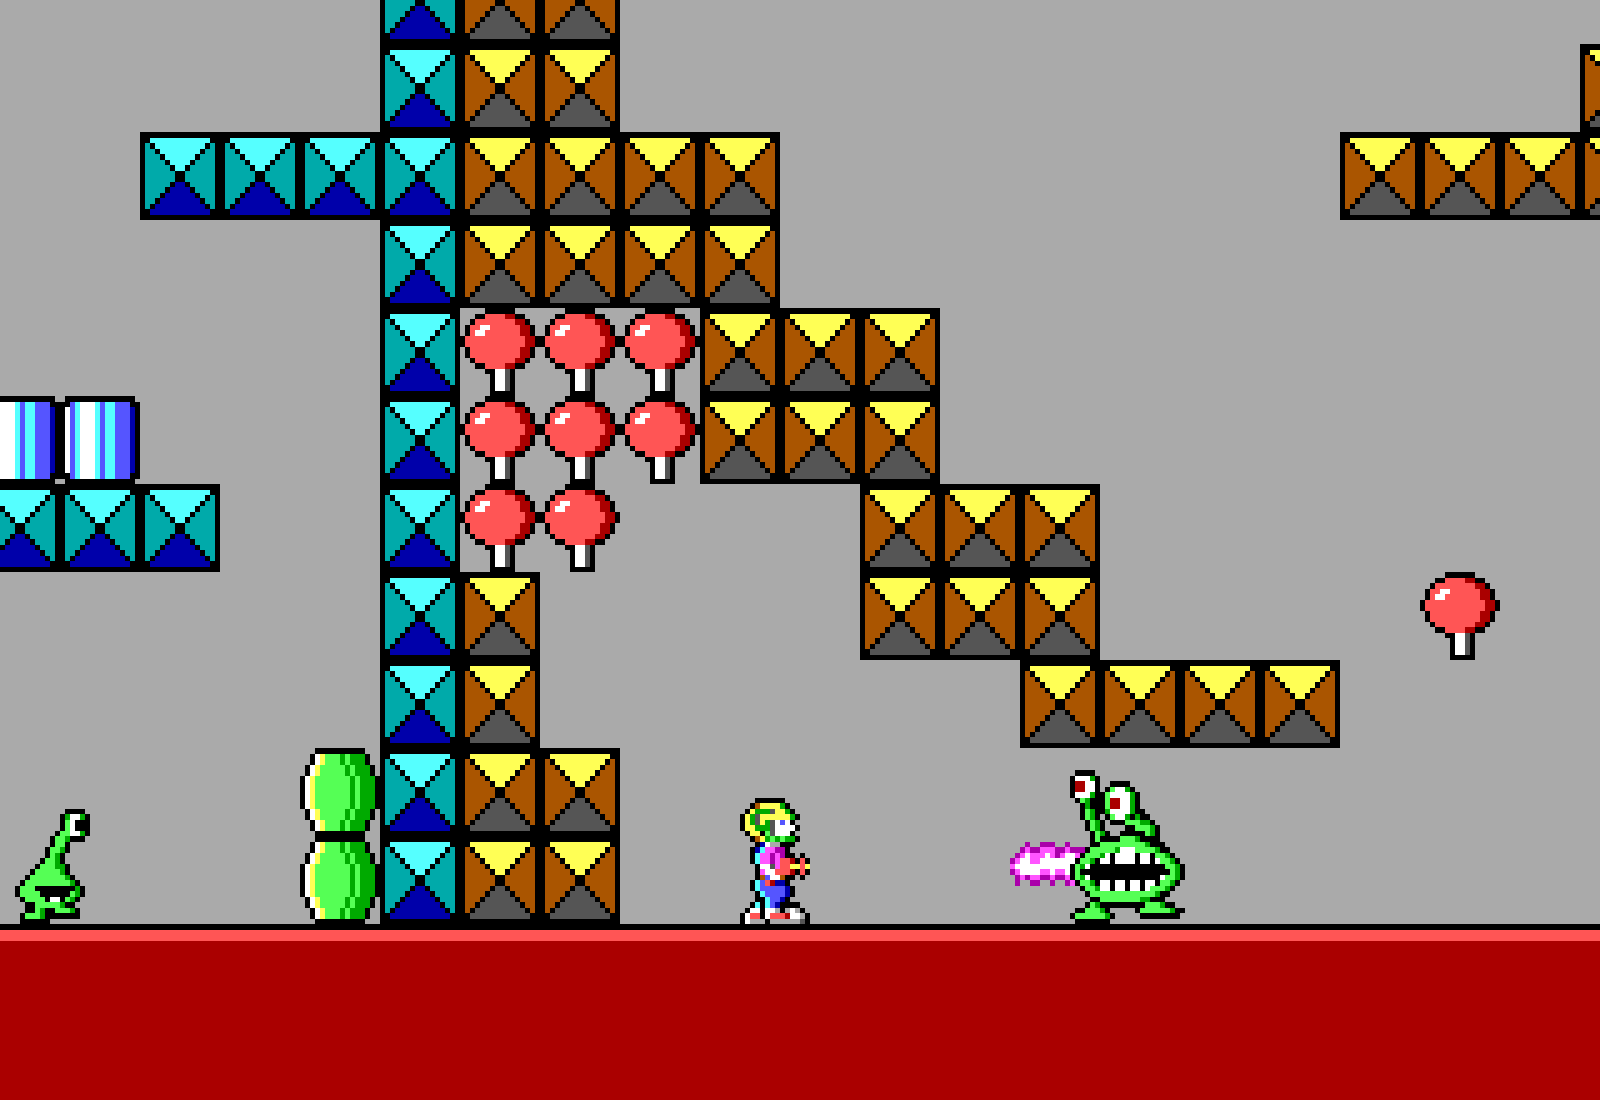
\includegraphics[width=.95\textwidth]{screenshots_300dpi/Keen_Verticons_gameplay.png}
\end{subfigure}
\par\bigskip % force a bit of vertical whitespace
\begin{subfigure}[b]{\textwidth}
  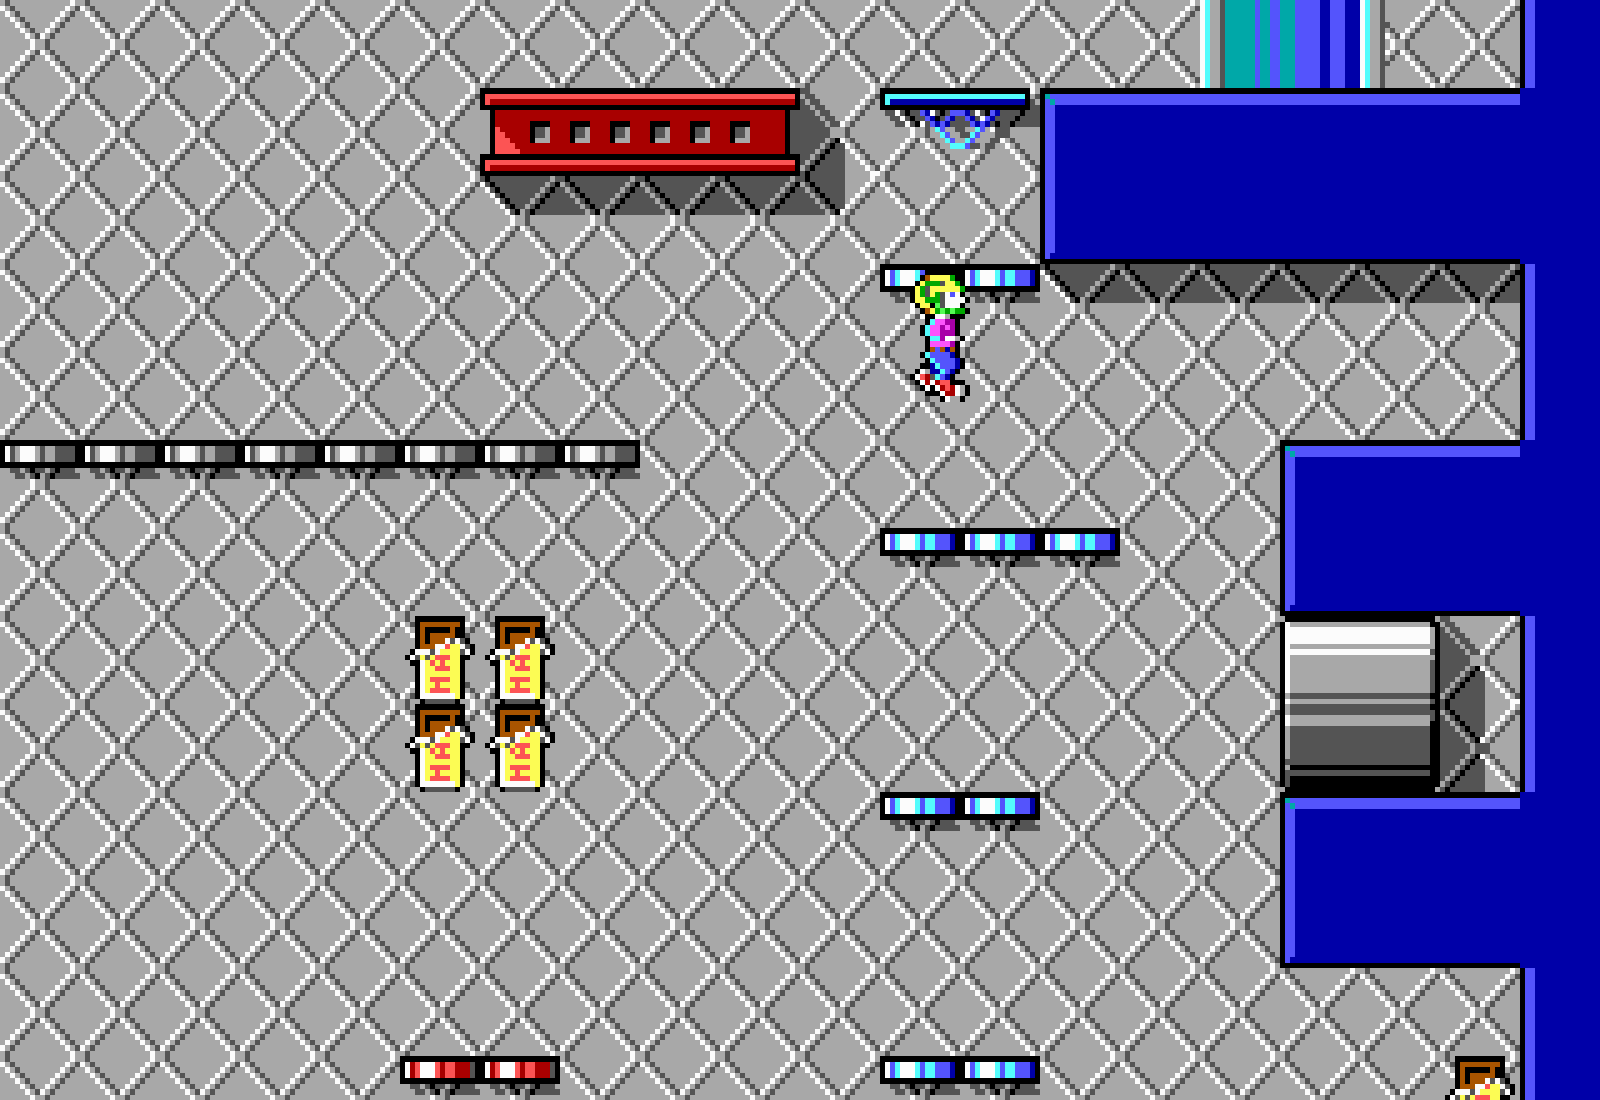
\includegraphics[width=.95\textwidth]{screenshots_300dpi/keen1_2.png}
\end{subfigure}
\caption*{Keen I - \textit{Marooned on Mars} (above) and Keen II - \textit{The Earth Explodes} (below).}
\end{figure}
 
\begin{figure}[H]
\centering
\begin{subfigure}[b]{\textwidth}
  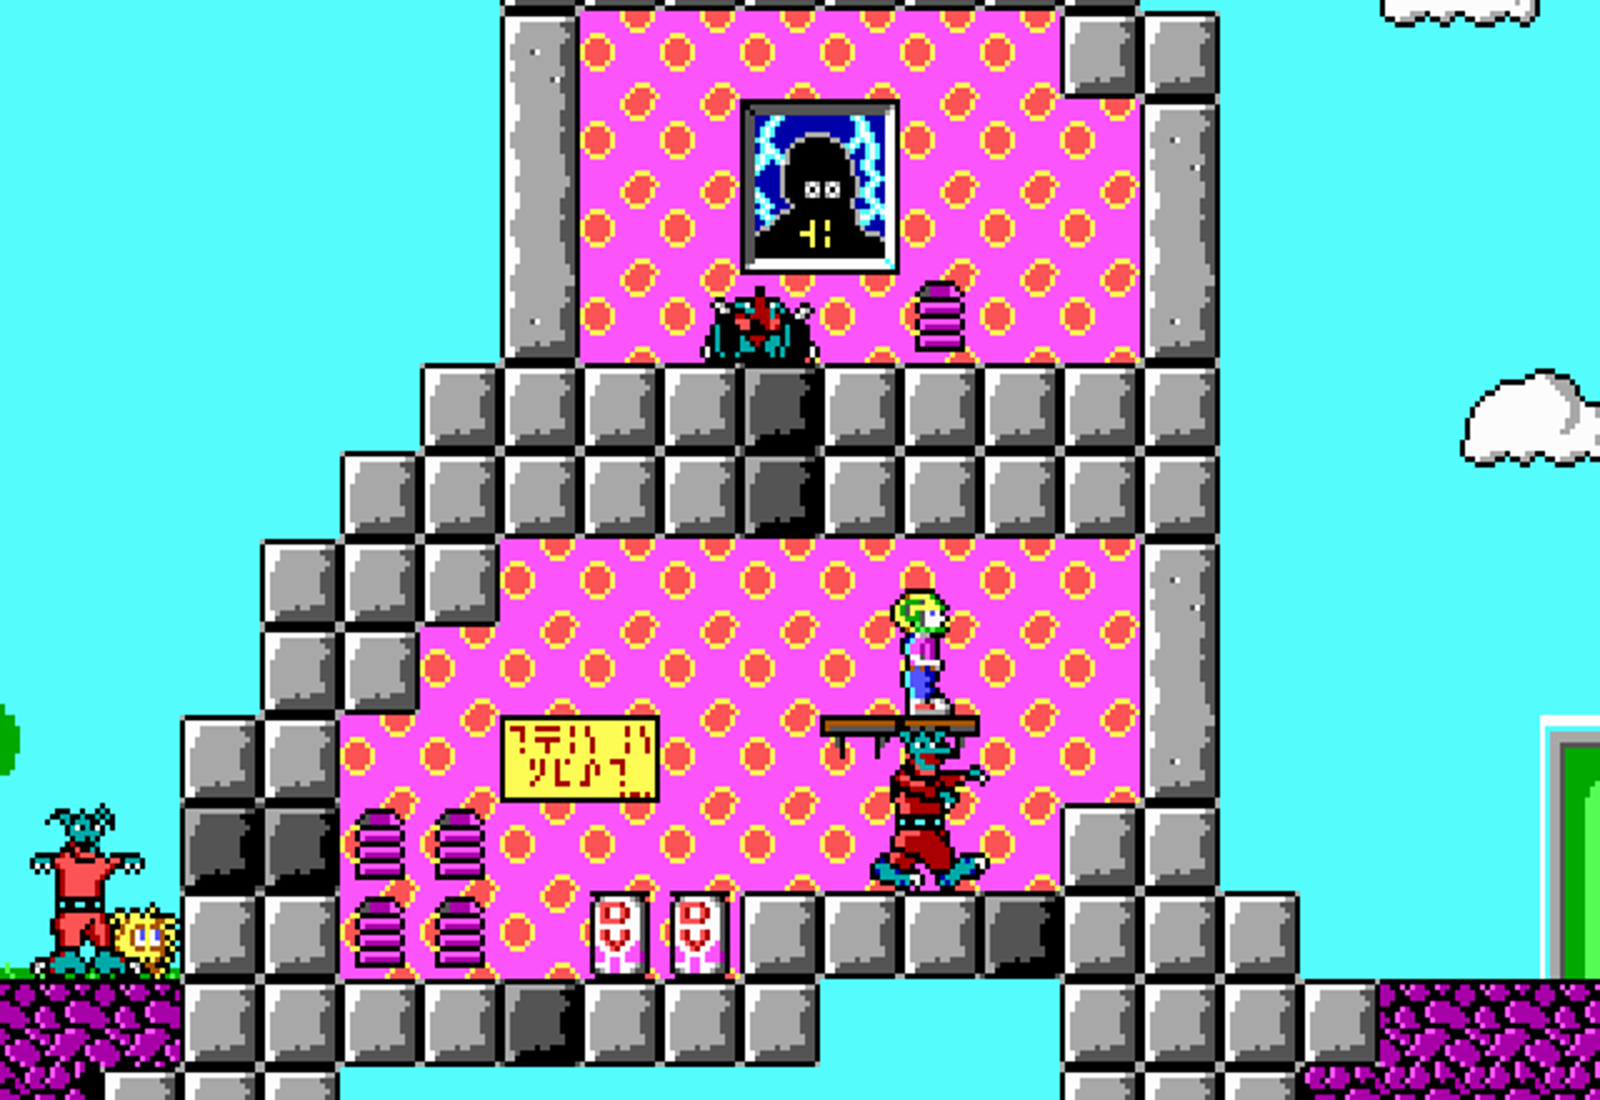
\includegraphics[width=.95\textwidth]{screenshots_300dpi/keen1_3.png}
\end{subfigure}
\par\bigskip % force a bit of vertical whitespace
\begin{subfigure}[b]{\textwidth}
  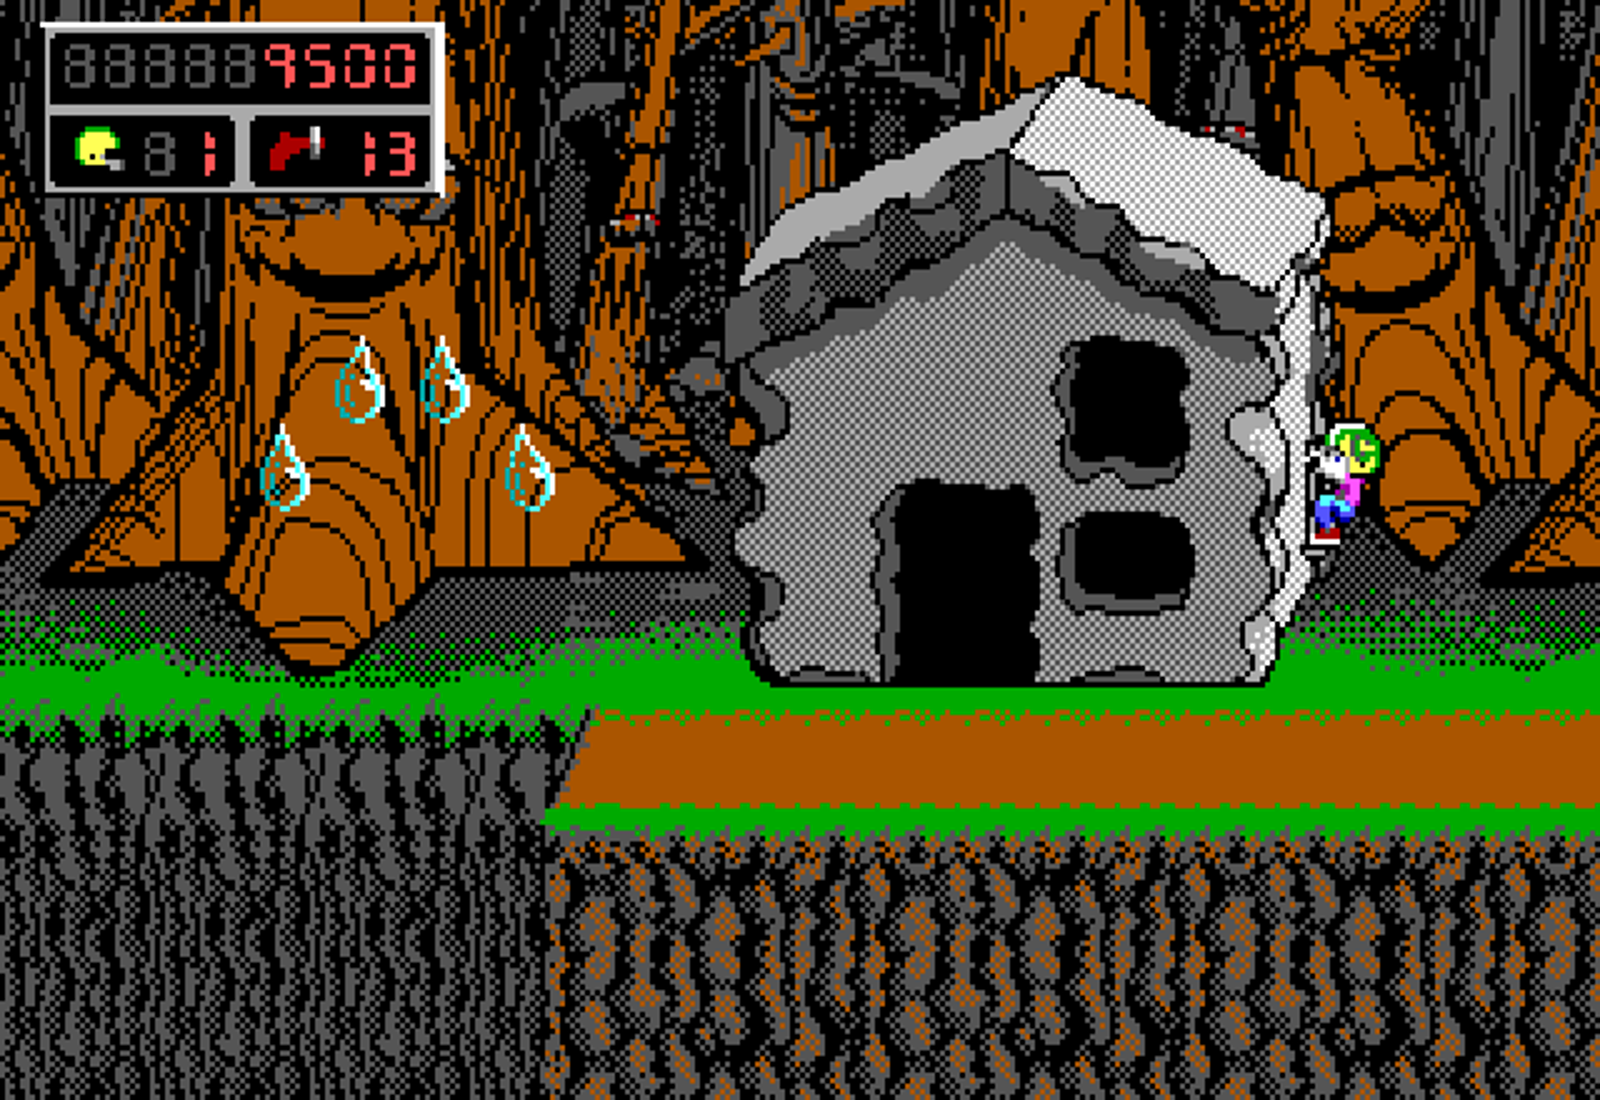
\includegraphics[width=.95\textwidth]{screenshots_300dpi/keen2_1.png}
\end{subfigure}
\caption*{Keen III - \textit{Keen Must Die!} (above) and Keen IV - \textit{Secret of the Oracle} (below).}
\end{figure}  


\begin{figure}[H]
  \centering
  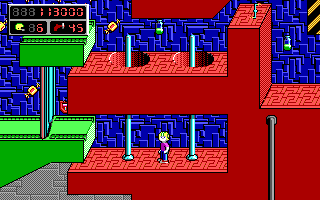
\includegraphics[width=.95\textwidth]{screenshots_300dpi/keen2_2.png}
  \caption*{Keen V - \textit{The Armageddon Machine.}}
\end{figure}


\par
When their boss and owner of Softdisk, Al Vekovius, confronted them on their plans, as well as their use of company resources to develop the game, the team made no secret of their intentions. Vekovius initially proposed a joint venture between the team and Softdisk, which fell apart when the other employees of the firm threatened to quit in response, and after a few weeks of negotiation the team agreed to produce a series of games for Gamer's Edge, one every two months. One of the games they developed to fulfill their obligation was \textit{Commander Keen in Keen Dreams}, which was released in June 1991.\\

\par
The second main game, \textit{Commander Keen in Goodbye, Galaxy}, was released in December 1991. It consisted of episodes four and five of the series, \textit{Secret of the Oracle} and \textit{The Armageddon Machine}, where \textit{Secret of the Oracle} was released for free, and the other episode sold by Apogee.\\

\par
The final id Software developed game was \textit{Commander Keen in Aliens Ate My Babysitter}, also released in December 1991. Originally planned to be the third episode of \textit{Goodbye, Galaxy} and sixth episode overall, the team decided to published it as a retail title through FormGen.\\

\begin{figure}[H]
  \centering
  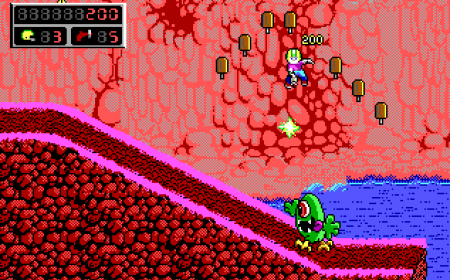
\includegraphics[width=.95\textwidth]{screenshots_300dpi/keen3_1.png}
  \caption*{Keen VI - Aliens Ate My Babysitter.}
\label{fig:keen_1}
\end{figure}


\trivia{Even though this is the last game in the series, this was not the last one to be created. \textit{Commander Keen 5: The Armageddon Machine} was created after \textit{Commander Keen 6: Aliens Ate My Baby Sitter!} because the latter had to go to retail and that required lead time.}\\

\par
Another trilogy of episodes, titled \textit{The Universe Is Toast}, was planned for December 1992; id Software worked on it for a couple of weeks, but then shifted the work to another game. The name of that new game was \textbf{Wolfenstein 3D}...

\end{document}